\documentclass[11pt]{article}

\usepackage[letterpaper,margin=0.75in]{geometry}
\usepackage{booktabs}
\usepackage{graphicx}
\usepackage{listings}

\setlength{\parindent}{1.4em}

\begin{document}

\lstset{
  language=Python,
  basicstyle=\small,          % print whole listing small
  keywordstyle=\bfseries,
  identifierstyle=,           % nothing happens
  commentstyle=,              % white comments
  stringstyle=\ttfamily,      % typewriter type for strings
  showstringspaces=false,     % no special string spaces
  numbers=left,
  numberstyle=\tiny,
  numbersep=5pt,
  frame=tb,
}

\title{Reliable Transport}

\author{Jonathan George}

\date{}

\maketitle

\section{Description}
For this project, we have implemented a reliable transport protocal based on TCP. The major components of this protocal include a sender window buffer, receiver acknowledment, and a resend timer. 
In this protocal, the sender first places all the data to send into a buffer. This buffer has a sliding window which keeps track of packets unsent, sent and acknowledged. 
The sender upon starting to send a packet will send all availible packets allowed by the window size. It will not send a packet which is more than the window size away from the lowest unacknowledged packet.
Whenever the receiver recieves a packet, it will store this packet in a buffer and sent an ack for the lowest segment it needs next. The receiver will store packets which are out of order, so if a single segment is missing it will catch itself up once it recieves that segment.
When the sender receives an ack for a message it will tell the buffer to slide the window to that ack number and send any newly made availible data within the new window space. 
The resend timer is reset everytime a packet is sent from the reciever side. It plays the role of a watchdog timer, watching for a dropped packet or too slow of a connection. When it expires, it will resend the lowest unacknowledged packet and wait again for a returning ack. When this ack arrives the sender will send all data availible based on that ack.

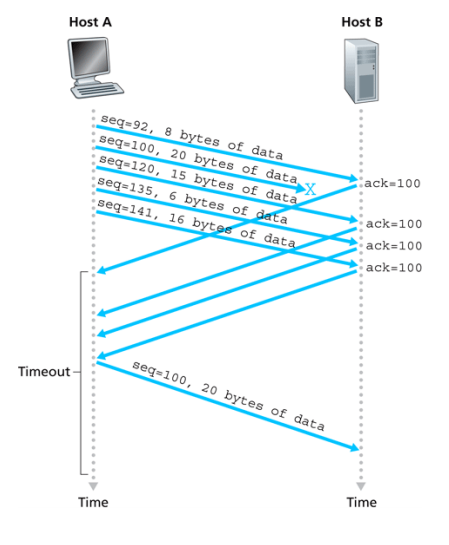
\includegraphics[width=11cm]{fast_transport.png}
Credit for image is given to Dr. Zappala's class slides.

\begin{lstlisting}
class Node:
    def __init__(self,scheduler):
        self.scheduler = scheduler

    def handle_message(self,t,message):
        print "Received at",t,':',message.body
        if message.times < 3:
            self.scheduler.add(t+1.5, message, self.handle_message)
        message.times += 1
\end{lstlisting}

\section{Section Name}

Mauris dictum augue a eros adipiscing mollis. Duis tempus, risus sed
iaculis vehicula, mauris mi aliquam odio, aliquet congue ligula tortor
vitae leo. In convallis, lectus sed egestas tincidunt, augue massa
lacinia augue, a ornare dui magna id enim. Fusce porttitor scelerisque
lorem nec eleifend. Cras lobortis eleifend orci, non lacinia felis
tincidunt eget. Nam vulputate tellus magna, at scelerisque
ligula. Duis dictum bibendum odio nec lobortis. Ut dignissim fringilla
euismod. In pharetra augue et odio blandit malesuada. Nulla lacus
nisi, auctor eget aliquet a, auctor at lorem. Suspendisse nec laoreet
sapien. Nulla facilisi. Nam a congue nunc. Pellentesque auctor turpis
ac augue aliquam convallis. Aenean sit amet eros nibh. Morbi a egestas
libero.

\vspace{0.5cm}
\begin{tabular}{lc}
  \toprule
  Setting & Result\\
  \midrule
  1 & 1.0\\
  2 & 3.45\\
  3 & 7.85\\
  4 & 15.89\\
  \bottomrule
\end{tabular}
\vspace{0.5cm}

Nam sed lacus sit amet nisl bibendum rutrum vel id nisl. Etiam sit
amet ipsum vulputate tellus fringilla tristique a et augue. Etiam
suscipit ante id est lobortis hendrerit. Vivamus vel nisl sit amet
metus volutpat faucibus. Praesent nunc urna, luctus vel convallis
eget, luctus et odio. Nunc et nisl felis. Fusce quis libero sit amet
libero cursus pretium. Vivamus dictum risus non tellus commodo non
bibendum tortor convallis. Cras tempor orci eu leo auctor sed euismod
arcu consectetur. In scelerisque felis et erat commodo
bibendum. Pellentesque hendrerit enim vitae neque sollicitudin
bibendum. In ligula lorem, blandit sit amet aliquet eget, accumsan ut
sem. Maecenas in velit justo. Morbi tellus sem, ultricies in tristique
non, aliquam a lacus. Sed rhoncus blandit ligula, ut eleifend magna
lacinia quis.

\begin{enumerate}

\item Item.

\item Another item.

\end{enumerate}

\section{Section name}

Donec luctus, libero et egestas tincidunt, arcu ante commodo nunc,
quis sodales leo risus non libero. Mauris ac blandit ligula. Praesent
in dolor non nibh congue blandit. Curabitur in sodales
neque. Curabitur tincidunt nisl nec mauris bibendum
molestie. Suspendisse non justo erat. Ut quis odio elit, sit amet
ullamcorper dui. Nam massa urna, tempus non hendrerit porttitor,
feugiat quis quam. Quisque lacinia cursus nulla, id placerat enim
accumsan et. Donec porta pharetra tincidunt.

\includegraphics[width=11cm]{graphs/download-combined}

\end{document}